\section{Neural Networks based view matching}

The second technique offered in this work is based on neural networks. This approach is not designed as a standalone method but is presented only as a proof of concept and further used in the 2-Stage approach presented in the chapter [TODO chapter reference]. The used neural network is inspired by siamese neural networks [TODO ref].\par
These networks usually consist of two parts and are typically designed to compare any two entities. The first part consists of two networks with the same structure and usually with shared weights. This part is used for the automatic feature extraction from the input entities. The second part consists of a single network taking feature vectors extracted by both neural networks in the first part, performing the desired operation on the entities, and building corresponding output. In the case of comparison network is the output of the second part, and therefore of the whole network, a single number between 0 and 1, determining the similarity of the entities. The typical structure of a siamese neural network is shown in Figure \ref{fig:siamseNetwork}.

\begin{figure}[htpb]
    \centering
    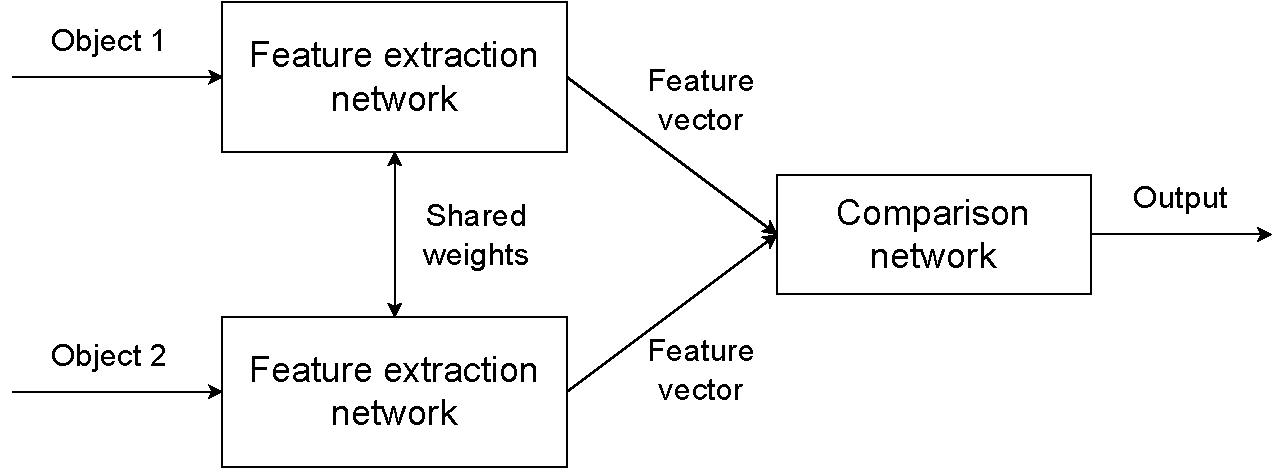
\includegraphics[width=0.8\textwidth]{siamseNetwork.pdf}
    \caption{Example of a siamese network used for object comparison} \label{fig:siamseNetwork}
\end{figure}

\subsection{Networks structure}

In this work, a slightly modified PointNet network, see chapter [TODO chapter ref], is used as a feature extractor. The only modification compared to the original networks is in the sizes of the layers and the output because we are typically working with significantly more sparse point clouds than the network designers\footnote{The exact parameters of the network are stated in the attachments [TODO add params to the attachment]}. As a result, the extracted feature vector contains only 256 numbers instead of 1024.\par
The feature vector extracted by this network is the scene template extracted from each input, processed in the future steps, and eventually stored in the storage.\par
The two extracted feature vectors are further compared by a single multilayer perceptron network (further MLP). This network has 512 input neurons and produces a single output. The network takes as input a concatenation of both feature vectors and produces a number between 0 and 1, describing the similarity of the scenes represented by given feature vectors. Several architectures of the networks were tried, but the best results were produced by a network with a single hidden layer containing 256 neurons and with a sigmoid as an activation function on the output neuron.

\subsection{Training of the networks}

Both networks are trained separately. For the training of the PointNet, used for the feature extraction, we used an original algorithm presented in [TODO reference]. In order to be able to evaluate the results and compare them with the expected results in the dataset, the PointNet network was concatenated with a simple MLP network used for the object classification. Then, the whole classification network was trained on the [TODO dataset link] dataset. After the classification network was trained, the final MLP network was removed, and the first PointNet part was used as a trained model for the feature extraction.\par
The second part of the network, namely the MLP comparing two feature vectors, was trained using a backpropagation algorithm [TODO ref] based on the mean squared error loss function [TODO ref]. The dataset was generated from a sample simulation, see chapter [TODO chapter ref]. During the simulation, the trained feature extractor network creates a feature vector from each scene. Afterward, a set of all pairs of the feature vectors is made. A random subset was chosen from this set, and all couples from this subset were labeled using exact scene locations received from the simulator and the criteria described in the chapter [TODO chapter ref]. This labeled subset was used as a training set for the MLP network.
